
\subsection{PHYSICS AND PROPERTIES OF SOLIDS}
The most common distinction between solids is taking their resistivity as a criterion. We can distinguish three main categories for them - metals, semiconductors and isolators. Within that we can also provide temperature differences beneath them as for the metals, the resistivity goes down with the temperature increase and for the rest of them it is quite the opposite.

Also, as it will be later extended, when we light a semiconductor or an isolator we can clearly observe so called \textit{absorption threshold}. This is directly connected to the inner energy structure of a material(solutions to the Schroedinger equation and their restrictions).

\begin{figure}[H]
\centering
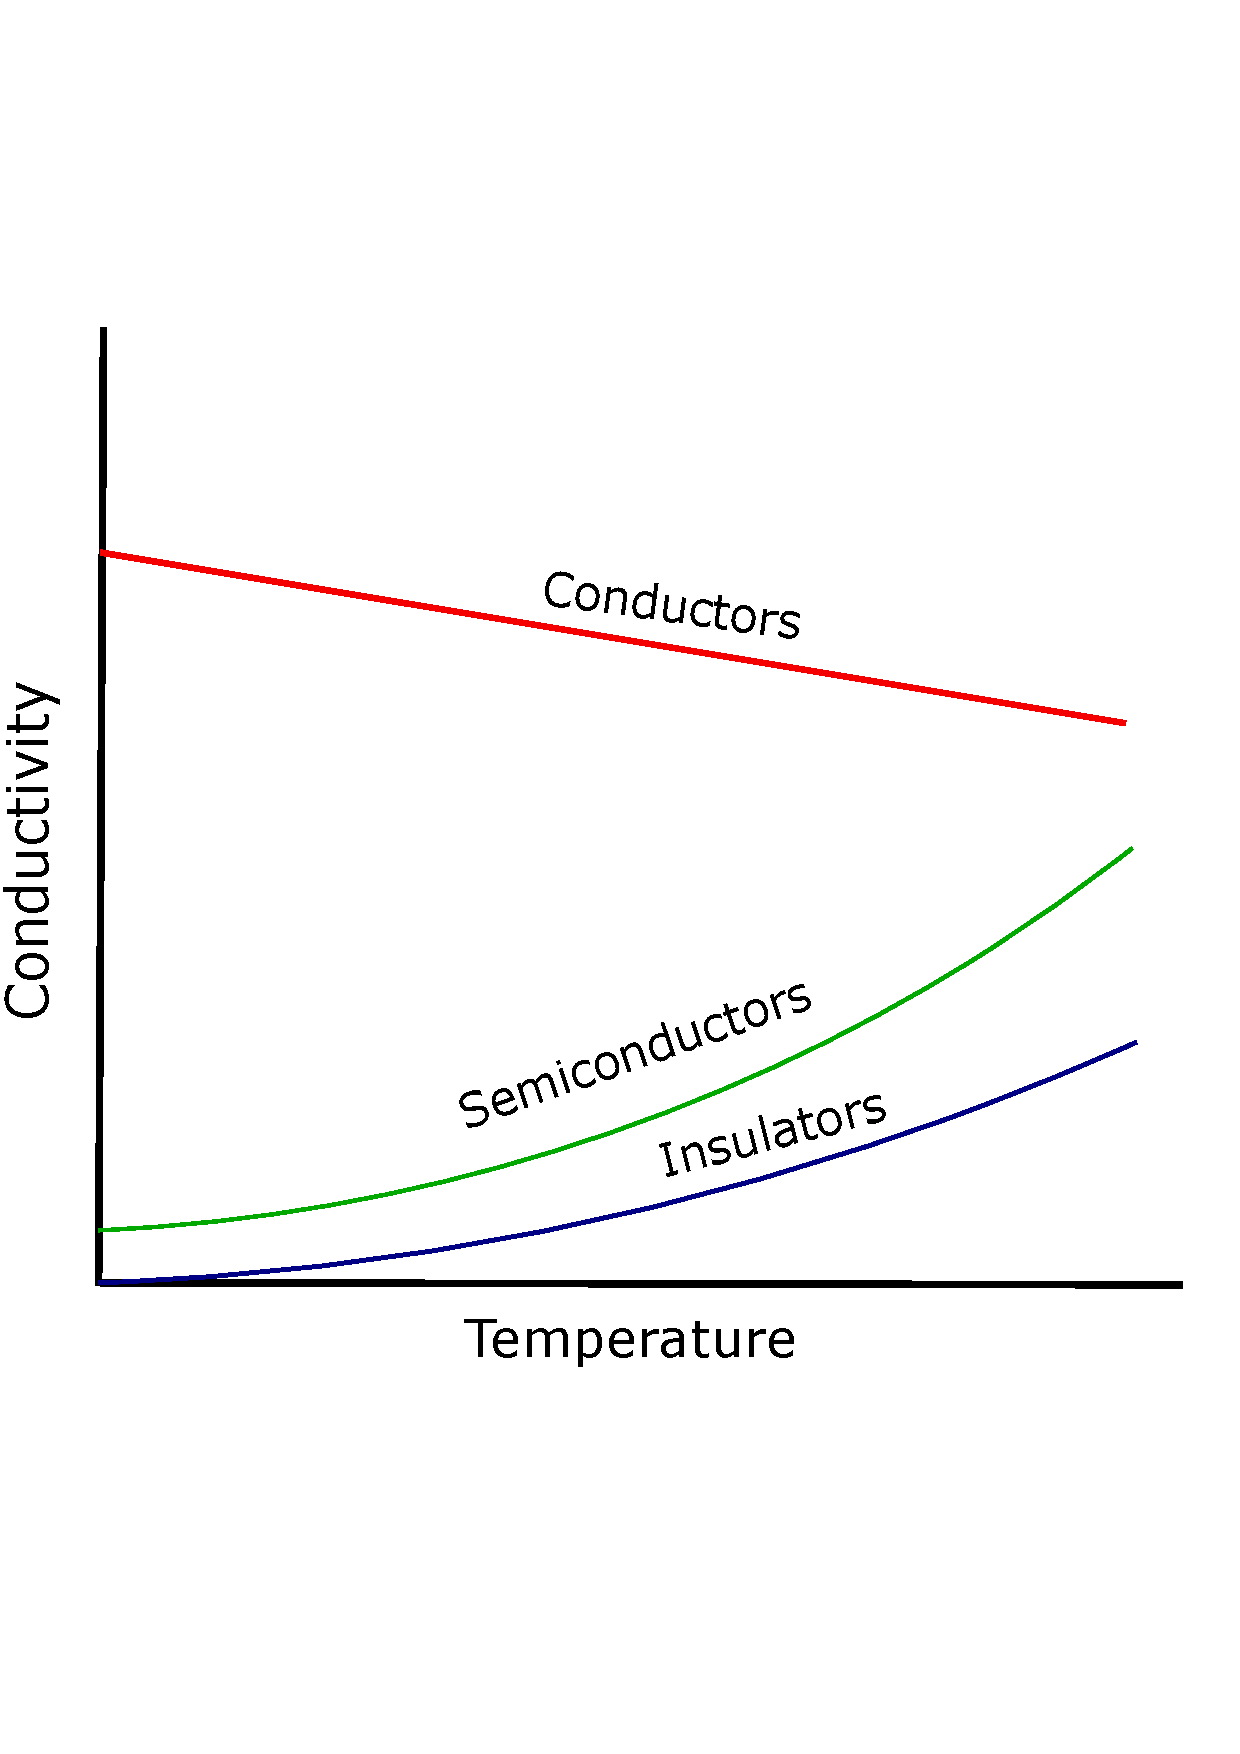
\includegraphics[scale=0.45]{Con_temp.pdf}
\caption{Demonstrations of conductivity behaviour of different types of solids}
\end{figure}

\subsection{DRUDE MODEL OF FREE CARRIERS}
The discovery of electron in 1897 had the great impact on the first attempt to describe properties of solids. Fairly early, just three years later, Drude constructed his first theory which based on the usage of quite successful kinetic theory, which described the behaviour of gases. Starting with metals he imagined a gas of electrons which are identical solid spheres moving randomly in straight lines. They change directions by collisions and of course no other forces than that of the very quick collisions are taken into account. As metals are neutral, Drude deduced that much heavier and steady particles are compensating negative electron charge. Strictly, that kind of model provides us with the crystal structure but back then, Drude assumed (and for great deal of metals it's fairly true), that only valence electrons are important and they move freely through the whole metal. The basic assumptions for the model are:

\begin{enumerate}
\item Between collisions, interactions electron-electron and electron-ion are able to be neglected. The first one is called \textit{independent electron approximation} and the second is called \textit{free electron approximation}. 
\item Only the collisions are important. They are approximately instantaneous events that alter the velocity of the electron. The electron-electron scattering is one of the least important scattering mechanisms in metals. Nevertheless with others, very often, in describing conducting electrons it is not important to describe all mechanisms deeply. 
\item We can assume that the period in which an electron isn't making any collision is $\tau$ \textit{(relaxation time)} and thus the probability that electron is undergoing a collision in any infinitesimal time period dt is $\frac{dt}{\tau}$. This of course means that $\tau$ is average time and it is independent of both velocity and position $\rightarrow$ therefore also time. 
\item Thermal equilibrium is achieved only through collisions.
\end{enumerate}

\subsubsection{Electrical Conductivity}

Drude model can describe, with certain accuracy, the Ohm's law $V=IR$. Resistance R is a quantity which is dependent of the dimensions of the material, therefore resistivity, which has been mentioned before can be used.

\begin{equation}
\mathbf{E}=\rho\mathbf{j}
\end{equation}

The current density \textit{j} is the same as in former section, when we were describing Maxwells equations. If n electrons move with velocity \textbf{v} in time period dt and through area A we get that charge connected with that quantities is $-nevAdt$ so current density is:

\begin{equation}
\mathbf{j}=-ne\mathbf{v}
\label{eq:curr_dens_drud}
\end{equation}

and is just a net current because of random electron movement. 
Also, let's assume that electron has a velocity $\mathbf{v_0}$ at time $t_0$ just after a collision and additional velocity $\frac{-\mathbf{E}e\tau}{m}$ from the external field, we can take average through long time period. The random velocity $\mathbf{v_0}$ disappears and therefore, connecting with \ref{eq:curr_dens_drud} we get that:

\begin{equation}
\mathbf{j}=\sigma\mathbf{E}
\end{equation}

\begin{equation}
\sigma=\frac{ne^2\tau}{m}
\end{equation}

This tells us about the linear dependence of \textbf{j} on \textbf{E}. Note that $\tau = \frac{m}{\rho n e^{2}}$ because $\tau = 1/\rho$ where $\rho$ is \textit{resistivity}.
Drude model was a first and simple model used in describing solid state materials. As simple as it is, it can yet provide some accurate results. Even more can be read in \cite{Aschcroft}


\subsection{CRYSTAL STRUCTURE AND BLOCH THEOREM}

To easily get to quantum dot description, we shall know that most materials used nowadays occur as crystals. They posses a so called translational order, which can be described by \textbf{Bloch theorem} and is a point group symmetry. The symmetry has its impact on most physical properties of a materials, therefore it is important to study if a material possess crystal symmetries. 

The Bloch theorem simply says that electron in a periodic potential V(\textbf{r}) can be described as 

\begin{equation}
\psi _\mathbf{k} (\mathbf{r}) = u_\mathbf{k}(\mathbf{r})e^i\mathbf{k}\mathbf{r}
\label{Bloch}
\end{equation}

where \textbf{k} is a wave vector and $u_\mathbf{k}$ has a periodicity of a crystal lattice so $u_\mathbf{k}(\mathbf{r}) = u_\mathbf{k}(\mathbf{r+R_n})$ and $\mathbf{R_n}$ is an arbitrary lattice vector.
The lowering of symmetry can provide optical anisotropy(optical properties are different in different directions) and lift degeneracies(provide more possible energy states in a system). Anisotropy is only found in solids.

\subsection{ENERGY STRUCTURE}
Bloch theorem \ref{Bloch} tells us more that a form a wavefunction. It also describes each electronic band(the effect of mixing atomic orbitals which provides the broadening in a discrete energy levels into so called bands). 

\begin{figure}[H]
\centering
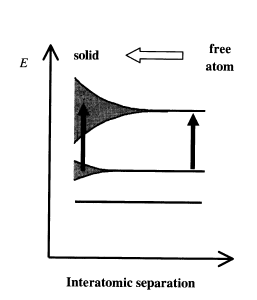
\includegraphics[width = 0.5\textwidth]{ch2/bands}
\caption{The broadening of energy levels as atomic orbitals cross each other when they are getting closer\cite{fox}}
\end{figure}

Optical transitions that are possible for distinct material and are available via \textit{selection rules} occur between each electronic band, of course if the beginning state is occupied and ending is empty. This \textit{absorption} is possible over a range of energies that are bigger than the gap between those levels. The energy structure is also widened because of the vibration bands that are possible because of the coupling between continuum of vibrational modes of the crystal and those electronic bands. What is important, those effects are also present in molecular materials such as QDs.

With the term of band formation, we cannot omit \textbf{the density of states}. It gives us the number of states that is possible to achieve in an abstract range of energies.

\begin{center}
\textit{number of states} in $[E,E+dE] = g(E)dE$
\end{center}


and is usually obtained from E(\textbf{k}) dependence

\begin{equation}
g(E) = g(k)\frac{dk}{dt}
\end{equation}

\subsection{BIGGER WORLD OF CARRIERS}
In reality of course, we cannot describe the carriers in the medium with such smooth potential like in metallic models. The potential periodicity that comes from the crystal periodicity gives us important informations about the behaviour of the electrons. The set of possible energies of an electron in periodic potential is quadratic $E=\frac{\hbar ^2k^2}{2m_e}$.


Also, in consequence of the Bloch law, being directly evaluated from the Schroedinger equation we have that:

\begin{equation}
\Psi _{n,\mathbf{k}}(\mathbf{r}) = \Psi _{n,\mathbf{k}+\mathbf{G}}(\mathbf{r})
\end{equation}

\begin{equation}
E_n(\mathbf{k})=E_n(\mathbf{k}+\mathbf{G})
\end{equation}

where \textbf{G} is a \textit{Reciprocal lattice} vector. 

\begin{equation}
\mathbf{G} = n_1\mathbf{b_1} + n_2\mathbf{b_2}+ n_3\mathbf{b_3}
\end{equation}

The periodicity of a crystal allows also to create \textit{The first Brillouin zone} which preserves that symmetry. We can also say that the number of available wavevectors in the I Brillouin zone is equal to the number of the primitive cells in the crystal volume.(the cells that with translation can reproduce the whole crystal)(This also means that one cell gives one possible \textbf{k} state, so we have 2N possible states when considering electron spin)

The electric current can flow through the body if the band isn't fully occupied by electrons. So we can say  that transport properties are indicated by the last electronic band, called Conduction band. To describe distinct potentials much easier it is usual to provide the concept of effective mass of a carrier in a band. 

\begin{equation}
m_e* = \left( \frac{1}{\hbar ^2}\frac{d^2 E}{dk^2}\right)
\end{equation}

and is a tensor in three dimensions. It can be noted that in the minimum of conduction band the effective mass is almost equal to the mass of a free electron. With that concept there comes another simple idea as well. Instead of using electrons in a band that's almost fully occupied(the Valence band)we can use the imaginary carriers - holes, which are the vacancies of an electron. To do it, we have to put it's mass and charge to be negative $ m_p * = -m_e * $ and it's momentum $k_p = - k_e$. So now we have energy of an electron in conduction band:

\begin{equation}
E(k) = E_c + \frac{\hbar ^2 k^2}{2m_e}
\end{equation}

and energy of a hole in valence band:

\begin{equation}
E(k) = E_v + \frac{\hbar ^2 k^2}{2m_p}
\end{equation}

After saying that, to calculate the concentration of carriers in thermodynamic equilibrium we have to consider the former introduced \textit{density of states} g(E) and the probability that the state will become occupied - \textit{the Fermi-Dirac function} f(E). For electrons:

\begin{equation}
n_0 = \int _{E_c}^\infty f(E)N(E)dE
\end{equation}

Because of the difficulty and the complexity of g(E) it is usually calculated numerically. Few facts can be said before though:

\begin{itemize}
\item inside the band gap g(E) = 0
\item in three dimensions $g(E) \propto \sqrt{E-E_c}$
\item inside the band g(E) is non-analytic(infinities from the derivative - Van Hove singularities) 
\end{itemize}

Here, we will also state the Fermi-Dirac distribution function:

\begin{equation}
\frac{1}{1+e^{(E_c-E_F(T=0K)/kT)}}
\end{equation}

Where $E_F$ is a Fermi level - the highest possible energy for electrons to posses at absolute zero temperature, (also chemical potential). Very often in intrinsic semiconductors it is called $E_i$.

\begin{figure}
\centering
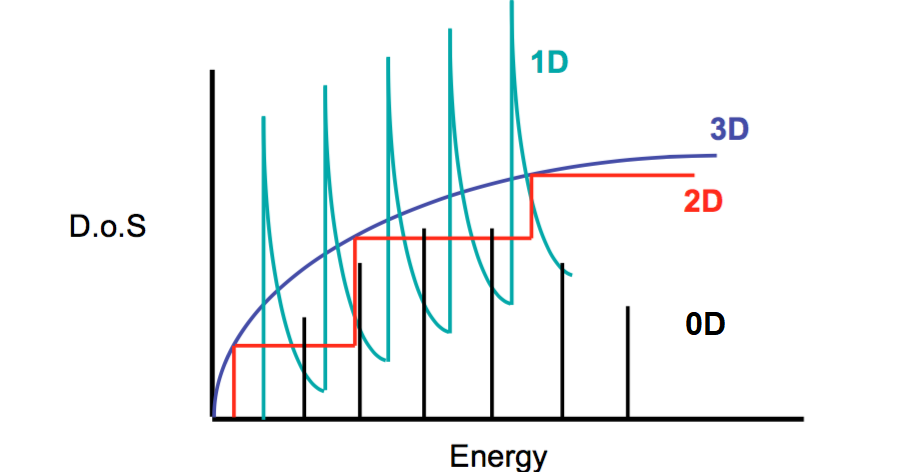
\includegraphics[width = 0.7\textwidth]{ch2/DOS}
\caption{Density of states behaviour\cite{DOS}}
\end{figure}

In intrinsic semiconductors(without any impurities) number of electrons in conduction band is equal to the number of holes in valence band because the electron excitation leaves exactly one vacancy behind. It is illustrated in Fig. \ref{intrin}

\begin{figure}
\centering 
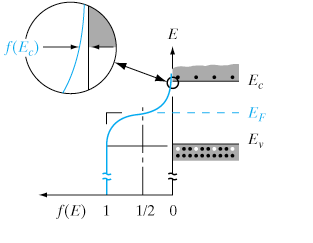
\includegraphics[width = 0.7\textwidth]{ch2/intrin}
\caption{Band diagram for intrinsic semiconductor and Fermi-Dirac function in $T>0K$ - there is a possibility that electron will be excited to higher state \cite{popko}}
\label{intrin}
\end{figure}

In all semiconductors in thermal equilibrium we have:
\begin{equation}
n_0p_0 = n_i^2
\end{equation}

The concept of an intrinsic semiconductor is rather idealistic so in reality, the crystal of a semiconductors has defects, usually intentional. We can have donor(more electrons than original atom) and acceptor(less electrons than original atom) impurities so it creates another donor or acceptor energy levels for carriers to jump easier into. For type n semiconductor, the current flow is mostly due to electrons and for type p due to holes.

\begin{figure}
\centering
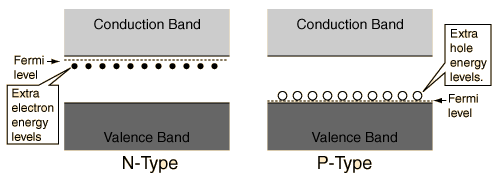
\includegraphics[width = \textwidth]{ch2/dban}
\caption{For p-type material(right) we can excite valence band electrons into acceptor state easier so we have holes in the valence band and for n-type material(left) we can extract electrons from the donor level and have carries in the conduction band\cite{hyper}}
\end{figure}

As a result of the placement of Fermi level in non-intrinsic semiconductors when comparing with the Fermi level of an intrinsic one, the equilibrium concentration is:

\begin{equation}
n_0=n_ie^{(E_F-E_i)/kT}
\end{equation}

\begin{equation}
p_0=p_ie^{(E_i-E_F)/kT}
\end{equation}

\subsection{NON-EQUILIBRIUM EFFECTS AND CARRIER INJECTION}

In all semiconductor physics most phenomena are based on non-equilibrium effects. With the chaotic thermal movement of the carriers, there's also effect of applying electric field to the semiconducting sample. The chaos of course cancels all components of the currents so no net mean velocity is present. The resulting current is therefore only the effect of applied field and is described using quantity called \textit{\textbf{carrier mobility}} $\mu =\frac{\langle v \rangle }{\epsilon }$. Where $\epsilon$ is the electric field and $\langle v\rangle $ is the average velocity. When also including holes in the transport we get:

\begin{equation}
\mathbf{J} = q(n\mu _e + p\mu_p)\mathbf{\epsilon}
\end{equation}

where q is the electric charge and n,p are electron and holes concentrations respectively.

Application of the electric field also changes the band diagram of the structure. Let's say we put electric field in the x direction. Then the force is equal:

\begin{equation}
F = -q\epsilon = -\nabla E_p
\end{equation}

where $E_p$ is the potential energy in this conservative field. Then:

\begin{equation}
\epsilon = \frac{1}{q}\frac{dE_p}{dx} \equiv - \frac{dV}{dx}
\end{equation}

and V is the electric field potential. 

\begin{figure}[H]
\centering
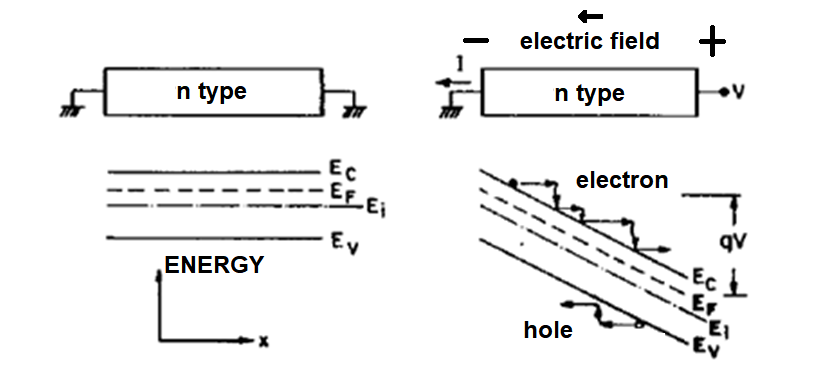
\includegraphics[width=\textwidth]{ch2/afield}
\caption{Band diagram for n type semiconductor when in equilibrium(left) and applying field(right)\cite{popko}}
\end{figure}

If the concentration changes, the uniformity isn't preserved. Then, the gradient of a concentration creates it's own current. It is called the \textit{diffusion current} and is equal:

\begin{equation}
J_{n_{diff}} + J_{p_{diff}} = qD_e\frac{dn(x)}{dx}-qD_p\frac{dp(x)}{dx}
\end{equation}

$D_{n(p)}$ is a diffusion coefficient and is connected to the mobility via Einstein equation so that: $D_{n(p)}=\mu _{n(p)} kT/q$. Notice both that holes and electrons move in the other direction the concentration gradient, but because of the negative value of electron charge both of currents are in the opposite directions. 

Carrier injection is connected to the situation where the excessive carriers are created in order of applying electric field or applying light on a sample. Then $np \ge n_i^2$. After the injection process, there occurs an undesirable effect in the photovoltaic physics - \textbf{\textit{recombination}}.

We can say that there are three processes of recombination in the bulk:
\begin{itemize}
\item Radiative(interband) recombination - electron loses energy by emitting photon with wavelength similar to the energy difference between bands.
\item Defect levels - Shockley-Read-Hall recombination. Electron or hole can be either trapped in additional defect energy state inside the band gap or if the carrier jumps to the energy state before thermal re-emission occurs. 
\item Auger recombination - involves extra two carriers, when recombination of one hole and one electron produces energy to excite third carrier higher in the band. 
\end{itemize}

More about recombination will be said   concerning quantum dots.\cite{popko} \cite{pv}

\subsubsection{QUASI-FERMI LEVELS}
It is worth to be noted now, that when in equilibrium the thermal generation of carriers is compensated by the recombination processes so equilibrium concentrations of both electrons and holes don't change on their own. The situation changes drastically when we provide the light source to create the light-induced carrier generation. Then, concentrations n and p will increase. Providing that excessive concentrations for holes and electrons are the same(no traps are included) we can calculate the non-equilibrium carrier concentrations as:

\begin{equation}
n = n_ie^(F_n-E_i)/kT
\end{equation}

\begin{equation}
p = n_ie^(E_i-F_p)/kT
\end{equation}

where $F_n$ and $F_p$ are quasi-Fermi levels of electrons and holes receptively. Their shift from $E_F$, induced by excessive carriers, is the way to distinguish how the equilibrium concentrations have changed. 
\subsection{SEMICONDUCTOR JUNCTIONS}

After stating previous information, let's imagine now that we connect two semiconducting materials together(no matter what technique with). Both of them have its own Fermi level. Then, after connecting them, the Fermi level gradient becomes $\frac{dE_F}{dx}=0$. If, additionally, we provide the non-equilibrium process, such us electric field or light induced carrier injection, the quasi-Fermi levels gradients become non-zero. For electron current only, induced with gradient concentration and electric field polarisation in the x direction we get: 

\begin{equation}
J_n(x) = q\mu _n n(x)\epsilon (x)+ qD_n\frac{dn(x)}{dx}
\end{equation}

Then after taking the excessive concentrations with quasi-Fermi levels included we get:

\begin{equation}
J_n(x) = \frac{\sigma _n (x)}{q}\frac{dF_n}{dx}
\end{equation}

where we can see that net current is strictly connected with the gradient of quasi-Fermi level. (Same can be done for holes)

\subsubsection{P-N JUNCTION}
A quick insight into p-n junction physics shall be put as it is in the principles of photovoltaic physics. Nevertheless, it would be just a reminder to the concept and more information can be obtained from f.e \cite{sze}
After connecting two semiconductors together, we know that for the equilibrium to be conserved our Fermi level gradient has to be 0 through the sample. This creates the difference in the energy structure which is called the built-in  potential $\Phi _{bi} = \Phi _n - \Phi _p$(because both of the Fermi levels must adjust to each other), where $\Phi _{n,p}$ is potential connected with the n or p type semiconductors respectively. For this to occur, because of the concentrations gradient between both materials, some of the electrons must go to the p type semiconductor, leaving volumetric positive charge behind. The holes from the p type "behave" the same way. This also explains the built in potential and creates the electric field between two sides called the\textbf{ depletion region}. Because of the equilibrium $n_{n0}p_{n0}=n_{p0}p_{p0}n_i^2$ (the first letter states the side of the sample) we can calculate the built in potential by using the concentration with:

\begin{equation}
\Psi _{bi} = \frac{kT}{q}ln(\frac{p_{p0}}{p{n0}})=\frac{kT}{q}ln(\frac{n_{n0}}{n{p0}})
\end{equation}

The width of a depleted region, the sizes for n and p types and potential distribution inside are usually calculated by assuming the box shape of the region. Because the electric field far from the junction must be zero the total negative electric charge density which was created in p-type must be equal to positive charge density in the n type. Therefore we can say that:

\begin{equation}
N_AW_p=N_DW_n
\end{equation}

where $N_{A,D}$ are acceptor and donor atoms concentrations and $W_{p,n}$ are lengths of box-approximated parts of the depleted region for p and n typ, see Fig.(\ref{fig:pn}). From Poisson equation we can calculate further each of the quantities \cite{sze}.

\begin{figure}
\centering
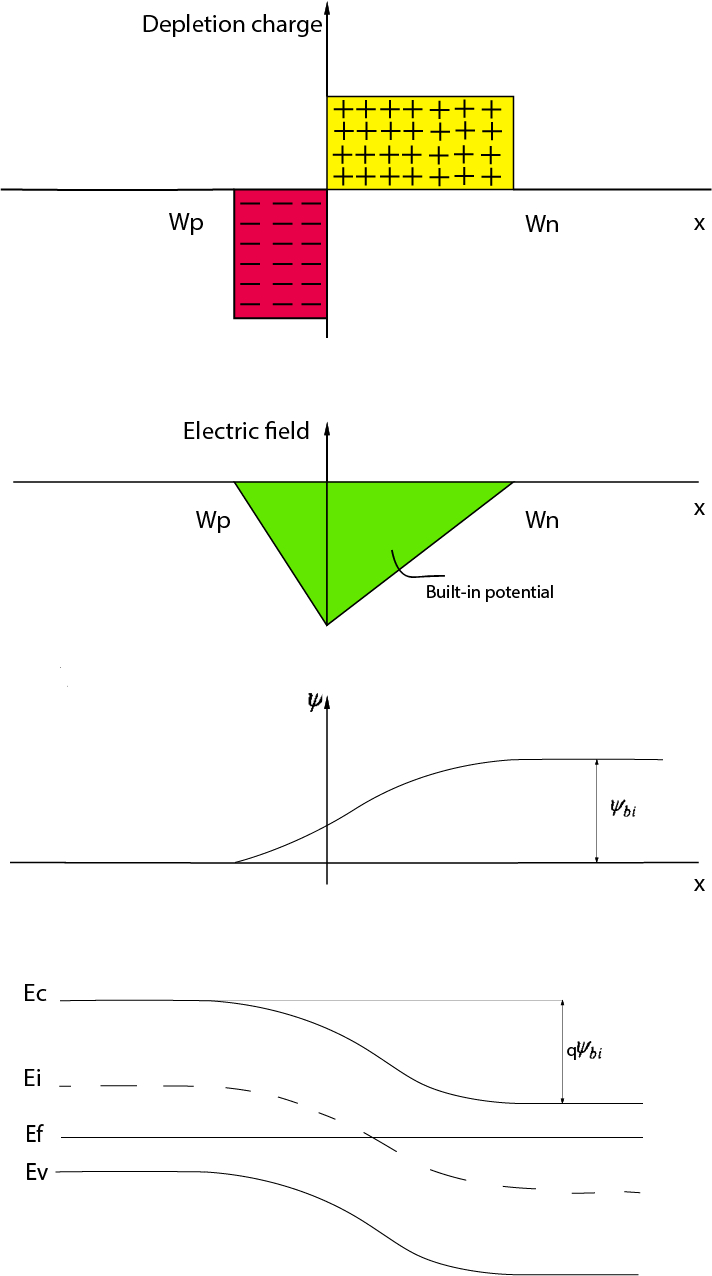
\includegraphics[width=0.6\textwidth]{ch2/pn}
\caption{Schematics of space-charge distribution, electric field in the depleted region, potential distribution and energy structure of a p-n junction in thermal equilibrium}
\label{fig:pn}
\end{figure}

From that all we can derive the Shockley diode equation for the total current density\cite{pv}

\begin{equation}
J = J_0(e^{\frac{qV}{kT}}-1) - J_{sc}
\end{equation}
